\chapter{Experiment}\label{ch:exp}
The experimental procedure is explained in Section \ref{sec:exp.proc}. 
It is discussed what experiments can be done in order to investigate closed-loop stability and the tracking performance of nonlinear geometric control.
In addition, a comparison is made between the performances of the nonlinear geometric controller and a linear \a{lqr} controller.

The controllers are tested on their ability to track a desired load trajectory. 
Section \ref{sec:exp.traj} presents several desired load trajectories that create different challenges for load position tracking, and it is discussed what could be expected from these experiments.

%***************************************\\
%Bart: Challenge of what? control challenges?\\
%Nam: challenges for load position tracking, beter?
%
%***************************************\\
%in what way a comparison can be made between the performance of the controllers.
In Section \ref{sec:exp.setup} the experimental setup is discussed. 
The model parameters for the \a{qr}-load system are presented, as well as the controller parameters for both nonlinear geometric controller and \a{lqr} controller.
The notion of a backstepping command filter is made to explain a mathematical simplification in the experiments.

Finally, in Section \ref{sec:exp.results} the results that are obtained from the load trajectory tracking experiments are presented and discussed.
The stability of the closed-loop system is demonstrated by using the nonlinear geometric controller and the differences in linear- and nonlinear controller performance are discussed.

\newpage
\section{Procedure}\label{sec:exp.proc}
The goal of the experiments is to analyze the controller performance and closed-loop stability in a load position tracking task.
The load positions are described by smooth trajectories $ x_{L,d}(t) $ in order to get well-defined control functions.
%, which is required to be smooth for geometric control, such that feed forward terms can be generated and implemented. 
In this work the desired load paths are generated manually. 
The corresponding required velocity and acceleration are calculated by a \textit{command filter}, which is explained in more detail in Section \ref{sec:exp.setup}.
For the purpose of load transportation, both controllers can be used. The difference is in the definition of the problem.

As described in Chapter \ref{ch:control}, the stability of the nonlinear geometric controller is evaluated by analyzing the error functions to check whether 1) the zero equilibrium of the closed loop tracking error $(e_x,e_v,e_q,e_{\dot{q}},e_R,e_\Omega)=(0,0,0,0,0,0) $ is exponentially stable and 2) the tracking errors $ \Psi_R $ and $ \Psi_q $ are bounded by an exponential decay function and the maximum error.
Performance of both nonlinear geometric control and \a{lqr} control are evaluated by comparing their ability to track a load trajectory with minimal error. 
The differences based on response time, load tracking accuracy and peculiarities are analyzed and discussed.

A linearized model is obtained by assuming small angles of both load and \a{qr} around an equilibrium point. 
The model is obtained by assuming an equilibrium point such that the \a{qr} is in a hover position with the load hanging directly underneath it.
The \a{lqr} cost function allows control of the states that define the \a{qr} position, \a{qr} attitude and load attitude by calculating the control inputs $ f $ and $ M $, in such a way that the system is stable. 
As a result, the linearized model does not allow direct reference tracking of the load position. 
%Therefore, full load position control is not possible. 
%This can be approached by \a{qr} position control and/or minimization of the load swing. 
This limitation illustrates an important difference between the use of a linear and a nonlinear model. 

The \a{lqr} controller in this thesis is designed to track a \a{qr} position and to minimize the load swing. 
The tuning of the \a{lqr} controller involves a trade-off between accurate \a{qr} movements and minimal load swing. 
%The controller will apply reference tracking of t
The \a{qr} position is based on the same desired load trajectories that are used for the nonlinear geometric controller. 
When assuming small angles and minimal load swing, the \a{qr} position should be approximately a cable length above the predefined desired load position. 
Note that this will not allow a direct comparison of the load trajectory tracking performance, nevertheless this will illustrate important differences between the controllers. 
%
%are defined in a different way.
%with different ob
%in means of
%and allow conclusions to be made about the 
%in load attitude
%exposed to trajectories 
%where large angles are required to track fast maneuvers

% Since it is not possible for \a{lqr} to apply reference tracking for the load trajectory, 
%\a{lqr} is a linear optimal control strategy and will be used to compare its result to a nonlinear geometric controller.

\newcommand{\caseA}{71}
\newcommand{\caseB}{72}
\newcommand{\caseBB}{75}
\newcommand{\caseC}{78}
\newpage
\section{Trajectories}\label{sec:exp.traj}
%What observations can be made in order to adapt the controller properties that improve performance of the test cases.

This section discusses a number of cases that describe different load trajectories for the \a{qr}-load system.
The trajectories are generated to obtain responses and test stability of the closed-loop system. 
A description of the desired trajectory is given in each case and the challenges that are involved are discussed.
In order to define the nonlinear geometric controllers, geometric approach requires the desired load trajectory to be twice-differentiable, meaning that it is not capable of tracking a non-smooth trajectory. For this reason, all signals that are used to generate the trajectories start smoothly, similar to the shape of a \textit{sigmoid} function. More details on the construction of the signals can be found in Section \ref{sec:app.casec}.

\subsection*{Case A}
In the first case, a smooth step-like trajectory is generated to investigate the step response of the system.
The step response is a commonly used analysis tool to obtain information about the stability of a dynamical system.
A step function is used to investigate the effects of a sudden input to the system. 
Typical response properties that can be investigated are: rise time, overshoot, settling time and steady-state error.
The goal is to transport the load from a starting position to a final position along the y-axis. 

%A point of this discussion is that 
%
%Note that the \a{lqr} however is capable of keeping the system stable, in response to a regular step function. In practice 

%The load position controller outputs a commanded load attitude signal $ q_c $, see Equation \ref{eq:con.q}, 
%which is a function of $x_{L,d}, \dot{x}_{L,d} $ and $ \ddot{x}_{L,d} $. 
Figure \ref{fig:set.caseA} shows the desired load position, velocity and acceleration in the y-direction. 
The desired position, velocity and acceleration in x- and z-direction are zero.
It can be expected that the step response is only able to track a trajectory up to a limited steepness. 
The commanded acceleration in Equation \ref{eq:con.A} is required to be bounded, such that 
\begin{equation}\label{eq:set.acc}
\parallel (m_Q+m_L)(\ddot{x}_{L,d}+ge_3)+m_QL(\dot{q}\cdot\dot{q})q \parallel < B
\end{equation}
where $ B $ is a positive constant \cite{Lee2010}. 
%is a design parameter to guarantee Lyapunov stability \cite{Sreenath2013c}. 
This might result in large errors, and it must be investigated whether the system is able to maintain stable. 

%
%***************************************\\
%Bart: Bedoel je dat large errors kunnen optreden als eq. 3-1 niet waar is? dus > B. Waar is design parameter B van afhankelijk? Kun je B zelf "tunen" zodat je systeem minder snel instabiel wordt?\\
%Nam: Aangenomen dat je Equation \ref{eq:set.acc} bedoelt; nee. B is een positieve constante waarde, niet een tuning parameter. (verbeterd in de tekst) Vergelijkbaar met een voorbeeld over stabiliteit; Een functie is stabiel als er een waarde $ \delta $ bestaat, zodat $ \parallel x(t) -x_{equilibrium} \parallel < \delta$. Het gaat er om dat wanneer  Equation \ref{eq:set.acc} oneindig groot is (not bounded), dat $ A $ in Equation \ref{eq:con.A} oneindig groot wordt, en daardoor klapt $ q_c=\frac{A}{\parallel A\parallel} $ in Equation \ref{eq:con.q}.
%
%***************************************\\
\begin{figure}[h!]
	\centering
	\makebox[.49\textwidth][c]{{\includegraphics[width=.45\textwidth]{\dir{LPOSQRL-allxLd\caseA}}}}
%	\makebox[.49\textwidth][c]{\subfloat[][ \label{fig:AxLdplot}]{\includegraphics[width=.45\textwidth]{\dir{LPOSQRL-xLdesplot\caseA}}}}
	\caption{Desired load trajectory Case A, y-direction\label{fig:set.caseA}}
\end{figure}		

%***************************************\\
%Bart: Did you found out with Daniel why a steep step works with simple pid controllers?\\
%Nam: Waarschijnlijk.. $ e_v $ wordt instantaan oneindig.\\
%@PID: De gecalculeerde gewenste input wordt instantaan oneindig. De werkelijk response is gelimiteerd door het systeem. Een actuator zal zijn hoogst mogelijke output geven, maar 1 sample periode erna is dat al niet meer nodig, omdat $e_v $ dan weer gezakt is.  \\
%@NGC: load position controller berekent een commanded load attitude $ q_c=\frac{A}{\parallel A\parallel} $, waar $ A = -k_xe_x-k_ve_v+(m_Q+m_L)(\ddot{x}_{L,d}+ge_3)+m_QL(\dot{q}\cdot\dot{q})q $. 
%Als $ e_v \rightarrow\infty$, dan krijg je rotzooi. Het lijkt me dat de controller hierdoor niet meer goed gedefinieërd is. \\
%Verderop in een paper staat nog: \textit{Assumed that commanded acceleration is uniformly bounded such that} $\parallel (m_Q+m_L)(\ddot{x}_{L,d}+ge_3)+m_QL(\dot{q}\cdot\dot{q})q\parallel < B $. En dat is niet het geval wanneer er een keiharde step wordt toegepast.
%
%Voorlopige conclusie: \\
%#PID: controller berekent één sampletijd een oneindig hoge desired input, actuatoren zullen pieken, maar het systeem klapt niet (per se). \\
%#NGC: load position controller kan geen commanded state meer berekenen voor desired input, waarschijnlijk gaan de control laws hierdoor overhoop. \\
%Verder \cite{Bullo2005} geeft een voorbeeld voor trajectory tracking op $ \mathcal{S}^2 $: "Let $ t\mapsto r(t) $ be a twice-differentiable reference trajectory with bounded velocity ...". Wellicht dat met een steile smooth step en een limiet op inputs, dat $ q_c $ (en de rest van de controllers) wel goed gedefinieërd is?
%
%***************************************\\

%***************************************\\
%Bart: Also speed of response/ rise time is important or not? With high rise time it is easy to have no overshoot but mostly this is not desired behavior.\\
%Nam: Edited, please check
%
%***************************************\\

%***************************************\\
%Bart: You mentioned ""What could be expected from these experiments" --> I don't see the expectation for the step response om this paragraph\\
%Nam: Added. Compleet genoeg?
%
%***************************************\\
\newpage
\subsection*{Case B}


%To investigate the behavior of the system undergoing aggressive maneuvers
The nonlinear geometric controllers are expected to be able to deal with large angles in the \a{qr} attitude, allowing aggressive maneuvering.
This can be tested by describing the next trajectory as a sine wave, growing in amplitude over time, in the direction of one axis in \IF.
This will result in a increasing distance between the load positions at each end of the movement, requiring increasing velocities on both the \a{qr} and the load.
To achieve this, it can be expected that the \a{qr} requires large rotations. It is investigated whether the system is able to perform load position tracking while dealing with increasing \a{qr} rotations.
%attitude needs large angles 
%to fly in a large angle.
%It can be expected that the \a{qr} attitude angles are large to reach the desired velocities.

The trajectory is generated by the product of signals A and B, shown in Figure \ref{fig:set.sinecaseB}, of which the first signal is a sine and the second consists of a smooth step up and down. This product results in signal C, shown in the same figure, which is chosen to be the trajectory in the direction of the y-axis of \IF. 
Figure \ref{fig:set.caseB} shows the desired load position, velocity and acceleration in the y-direction. The desired position, velocity and acceleration in x- and z-direction are zero.
\begin{figure}[h!]
	\centering
	\makebox[.49\textwidth][c]{\subfloat[][Trajectory generation\label{fig:set.sinecaseB}]{\includegraphics[width=.45\textwidth]{\dir{LPOSQRL-sineCaseB\caseB}}}}	
	\makebox[.49\textwidth][c]{\subfloat[][Desired trajectory \label{fig:set.xLdB}]{\includegraphics[width=.45\textwidth]{\dir{LPOSQRL-allxLd\caseB}}}}
%	\makebox[.49\textwidth][c]{\subfloat[][ \label{fig:}]{\includegraphics[width=.45\textwidth]{\dir{LPOSQRL-xLdesplot\caseB}}}}
	\caption{Desired load trajectory Case B, y-direction\label{fig:set.caseB}}
\end{figure}			
%
%
%***************************************\\
%Bart: Misschien geldt dit voor al je cases: wetenschappelijk gezien wil je net wat meer info over je trajectories.  Iemand zou je experiment moeten kunnen nadoen. Ze zouden je trajectories kunnen digitaliseren, maar wat meer info over bijv. maximale snelheden en acceleraties zou denk ik netjes zijn om te geven. Je grafieken geven in iedr geval een helder beeld over positie, maar dus indirect in mindere mate info over vel en acc. Deze zijn ook belangrijk voor agressive manouvres.\\
%Nam: all cases desired load position/velocity/acceleration toegevoegd. Duidelijker en voldoende?
%
%***************************************\\

\subsection*{Case C}
%For this case a
%A trajectory is generated 
This case is generated in order to investigate the response on tracking multiple conditions at the same time.  
%such as sideways position tracking with high velocity, without losing height while tracking up and down motion. 
%this case describes the desired trajectory as follows.
The trajectory along the y-axis in \IF is described as a sine wave with an increasing and decreasing amplitude over time, similar to case B.
%, which will require changing and high velocities. 
While following this wave, the load is commanded to move along the x-direction, while tracking a sine wave in the z-direction.
%an increasing and decreasing height.
%has the shape of a sine wave that moves along the y-axis and varies in amplitude in the direction of the x-axis, while 
 %going up and down in the direction of the z-axis.
%Changing velocities are required to track 
The changing amplitude of the trajectory that moves from side to side, requires varying velocities to 'keep up' with the trajectory. \\
In this case it can also be expected that large \a{qr} rotations are required to track the changing amplitude of the sine wave and the varying velocities.
While doing so, the \a{qr} is expected to lose height due to the rotations.
It can be investigated how the close-loop system responds to the forward movement, while tracking a swinging motion and whether the controller can correct for the expected height loss, while simultaneously tracking the varying heights. 

%movement, while moving forward, up and down.
%How the system reacts on the changes in height
Figure \ref{fig:set.caseC} shows the desired load position and a three dimensional representation, which can be seen as a \textit{figure eight} increasing and decreasing in size. Figure \ref{fig:set.caseC2} shows the corresponding desired velocity and accelerations in all directions. 
\begin{figure}[h!]
	\centering
	\makebox[.49\textwidth][c]{\subfloat[][\label{fig:set.xLdC}]{\includegraphics[width=.45\textwidth]{\dir{LPOSQRL-xLdes\caseC}}}}
	\makebox[.49\textwidth][c]{\subfloat[][ \label{fig:}]{\includegraphics[width=.45\textwidth]{\dir{LPOSQRL-xLdesplot\caseC}}}}
	\makebox[.32\textwidth][c]{\subfloat[][ \label{fig:}]{\includegraphics[width=.32\textwidth]{\dir{LPOSQRL-xLdesplot1-\caseC}}}}
	\makebox[.32\textwidth][c]{\subfloat[][ \label{fig:}]{\includegraphics[width=.32\textwidth]{\dir{LPOSQRL-xLdesplot2-\caseC}}}}	
		\makebox[.32\textwidth][c]{\subfloat[][ \label{fig:}]{\includegraphics[width=.32\textwidth]{\dir{LPOSQRL-xLdesplot3-\caseC}}}}
	\caption{Desired load Position Case C\label{fig:set.caseC}}
\end{figure}
\begin{figure}[h!]
	\centering
	\makebox[.49\textwidth][c]{\subfloat[][\label{fig:}]{\includegraphics[width=.45\textwidth]{\dir{LPOSQRL-dxLdes\caseC}}}}
	\makebox[.49\textwidth][c]{\subfloat[][ \label{fig:}]{\includegraphics[width=.45\textwidth]{\dir{LPOSQRL-ddxLdes\caseC}}}}
	\caption{Desired load trajectory Case C\label{fig:set.caseC2}}
\end{figure}

%***************************************\\
%Bart: Which multiple disciplines? Do you mean Large QR rotations leads to less lifting force which might limit the tracking performance in z-direction\\
%Nam: Ik bedoelde eigenlijk, meerdere objectives. Hoge zijwaartse snelheden, terwijl het hoogte moet tracken. Indirect daarmee ook, testen of het hoogte kan houden terwijl de QR kantelt. Beetje herschreven, beter?
%
%***************************************\\
\clearpage		


\section{Setup}\label{sec:exp.setup}
\paragraph{Model and Control parameters}
The simulations are developed using Matlab$^\text{\textregistered} $ and Simulink$^\text{\textregistered} $ R2013b.
The model parameters to define the system are based on a Parrot$^\text{\textregistered} $ Bebop Drone 1, also used in a research by \cite{Cornelis2014}, see Table \ref{tab:set.par}. The maximum thrust per rotor defines the maximum total thrust and moment. $ m_L $ and $ L $ are chosen arbitrarily.
\begin{table}[h!]
	\centering
	\begin{tabular}{|l|ll|l|}
		\hline
		\textbf{Parameter}&\textbf{Value}&&\textbf{Description}\\
		\hline
		$ m_Q $&0.4& $ kg $&Quadrotor Mass\\
		$ l $&0.126& $ m $&Arm length from \a{qr} \a{cm} to rotor\\
		$ I_{xx} $&2.23$ \times 10^{-3}$&$kgm^2 $&Quadrotor Inertia about x-axis\\
		$ I_{yy} $&2.99$ \times 10^{-3}$&$kgm^2 $&Quadrotor Inertia about y-axis\\
		$ I_{zz} $&4.8$ \times 10^{-3}$&$kgm^2 $&Quadrotor Inertia about z-axis\\
    	$ f_{i,max} $&1.96 &$ N $&Maximum thrust per rotor\\
		$ m_L $&0.1 &$ kg $&Load Mass\\
		$ L $&0.7 &$ m $& Cable Length\\		
%		$ d $&&&Drag Constant\\
%		$ b $&&&Thrust Constant\\
%		$ c_{\tau_f} $&&& Constant	\\
		\hline		
	\end{tabular}
	\caption{Modeling Parameters}
	\label{tab:set.par}
\end{table}

In order to get a feel for realistic physical limits, these can be based on hardware data, which could be found on the web \footnote{\url{http://blog.parrot.com/2016/01/12/comparison-bebop-2-vs-bebop-drone/}\label{url:set.bebop}}. 
These values are shown in Table \ref{tab:set.par2}, and can be compared with the simulation results, in order to check whether the outcome is in the same order of magnitude of a real physical system.
\begin{table}[h!]
	\centering
	\begin{tabular}{|ll|l|}
		\hline
		\textbf{Value}&&\textbf{Description}\\
		\hline
		13 & $ m/s $&Maximum top speed\\
		2.5& $ m/s $&Maximum vertical speed\\
		30 &$ deg $&Maximum inclination\\
		\hline
	\end{tabular}
	\caption{Hardware Parameters for Bebop Parrot Drone 1}
	\label{tab:set.par2}
\end{table}

The chosen controller gains in Equations \ref{eq:con.M}, \ref{eq:con.Fpd} and \ref{eq:con.A} can be found in Table \ref{tab:set.gains}.
\begin{table}[h!]
	\centering
	\begin{tabular}{|l|l|l|l|}
		\hline
		%63 61 41
		\textbf{Gain}&\textbf{Case A}&\textbf{Case B}&\textbf{Case C}\\
		\hline
		% % % % % %
		$	k_R	$	&	0.9	&	0.9	&	0.9	\\
		$	k_\Omega	$	&	0.1	&	0.1	&	0.1	\\
		$	k_q	$	&	3.9	&	3.9	&	3.9	\\
		$	k_\omega	$	&	2	&	2	&	2	\\
		$	k_x	$	&	6	&	6	&	6	\\
		$	k_v	$	&	2.75	&	2.75	&	2.75	\\
		% % % % % %	
		\hline
	\end{tabular}
	\caption{Controller gains nonlinear geometric controller}
	\label{tab:set.gains}
\end{table}
\clearpage

\paragraph{Command Filtering}
% %ADD Pro Con Command filter
%Easy implementation. Less computational effort.
%Less accurate, because filters high frequency signals.
A consequence of a backstepping control approach, is that it increases the order of the commanded states. 
The controllers generate control laws that are a function of the commanded signals and their derivatives.
%, which are generated by the controllers in outer loops.
%In the control design, discussed in Chapter \ref{ch:control}, the load attitude controller generates a commanded QR attitude $ R_c $ and its derivative $ \dot{R}_c $. In the same fashion, the load position controller generates a commanded load attitude $ q_c $ and its derivative $ \dot{q}_c $. 
As can be seen in Chapter \ref{ch:control}, the control laws require the values $ R_c, \dot{R}_c, \ddot{R}_c, q_c, \dot{q}_c $ and $ \ddot{q}_c $.
%Calculating the 
Time derivatives of the virtual control variables may be quite complex and the calculation could result in high computational costs.
Instead of analytic differentiation of these terms, which can be tedious, these values can be obtained with the use of a \textit{Command Filter} \cite{Farrell2008,Farrell2005}. \\
% %CHECK nodig?
%https://www.researchgate.net/post/Sliding_Mode_controller_Vs_Backstepping_controller
The state space implementation of such a filter is 
\begin{equation}\label{key}
\begin{aligned}
\dot{x}_1 &= x_2\\ %dxc
\dot{x}_2 &= -2\zeta \omega_{n}-\omega_{n}^2(x_1-x_c^o)
%+\omega_{n1})x_3-(2\zeta\omega_{n1}\omega_{n2}+\omega_{n2}^2)x_2-(\omega_{n1}\omega_{n2}^2)(x_1-x_c^o)
\end{aligned}
\end{equation}
where $ x_c=x_1 $ and $ \dot{x}_c =x_2$. If $ x_c^o $ is bounded, the $ x_c $ and $ \dot{x}_c $ are bounded and continuous.\\
The transfer function from $ x_c^o $ to $ x_c $ is 
\begin{equation}\label{key}
\frac{X_c(s)}{X_c^o(s)}=H(s)=\frac{\omega_{n}^2}{s^2+2\zeta\omega_{n}s+\omega_{n}^2}
\end{equation}
%%%%Where 
which has a unity gain at low frequencies, $ \zeta $ is the damping ratio and $ \omega_n $ the undamped natural frequency. 

The result of a command filter is that the command signal is being pre-filtered by low pass filters and generates an estimation of the derivatives of the commanded signal. Backstepping command filters are implemented to compute $ \dot{R}_c, \ddot{R}_c,\dot{q}_c, \ddot{q}_c,\dot{x}_{L,d}$ and $\ddot{x}_{L,d} $. 

%The transfer function of the original commanded input signal $ X_c^o $ and the filtered output $ X_c $ has the form

%%%CHECK figure niet nodig?
%%See Figure \ref{fig:app.CF}.
%The filter has the following state space representation
%%CHECK waar dit ook alweer vandaan kwam. Reference in Djapic/Farell -> 3e order voor bacterieen ofzo

%where $ x_1 = x_c$, $ x_2 = \dot{x}_c$ and $ x_3 = \ddot{x}_c$, such that $ x_c $ is the filtered output. 
%The nonlinear state space representation of this filter is given by
%\begin{equation}\label{key}
%\begin{bmatrix}
%x_c\\
%\dot{x}_c
%\end{bmatrix}
%=
%\begin{bmatrix}
%q_1\\
%q_2
%\end{bmatrix}
%\end{equation}
%\begin{equation}\label{key}
%\begin{bmatrix}
%\dot{q}_1(t)\\
%\dot{q}_2(t)
%\end{bmatrix}
%=
%\begin{bmatrix}
%q_2\\
%2\zeta\omega_n\left( S_R\left\lbrace \frac{\omega_n^2}{2\zeta\omega_n}\left[ S_M(x_c^o)-q_1\right] \right\rbrace-q_2 \right) 
%\end{bmatrix}
%\end{equation}
%where $ S_M $ and $ S_R $ are functions that can limit the magnitude and rate. 
The implemented command filter is shown in Figure \ref{fig:set.cf}.
\begin{figure}[h!]
	\centering
	\makebox[\textwidth][c]{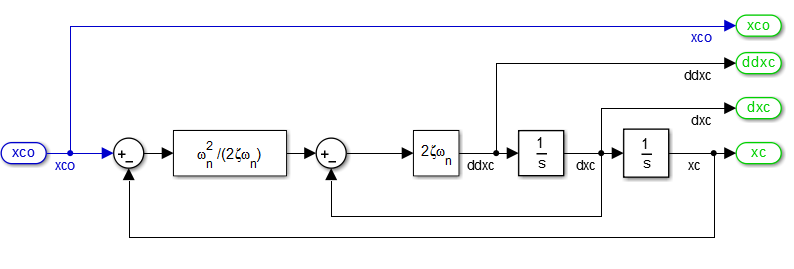
\includegraphics[width=.8\textwidth]{./StyleStuff/CFv2.png}}
	\caption{Command Filter\label{fig:set.cf}}
\end{figure}

%The chosen values for $ \omega_n $ and $ \zeta $ for the command filters are shown in Table \ref{tab:set.cf}. 
The parameters were determined by trial and error. 
The higher the value for $ \omega_n $, the higher the frequencies that are passed through the filter. 
Whenever the frequency was chosen too high, noisy derivatives are calculated, resulting in a destabilization of the system.
Choosing the values too low resulted in slow responses, and a bad estimation of the derivatives.
The damping ratio $ \zeta =0.98$, which results in a strong damping. 
For the experiments, $ \omega_n $ are $ 30,25,25 \frac{rad}{s}$ for the filtering of $ R,q,x_{L,d} $, respectively. 
\clearpage
%Limits for the magnitude and rates can be implemented, which is further explained in \cite{Borra2012}. 
%\begin{table}[h!]
%	\centering
%\begin{tabular}{|l|lll|}
%	\hline
%	& \multicolumn{3}{c|}{\textbf{Filter}} \\ \cline{2-4} 
%	& $ R  $     & $ q $      & $ x_{L,d} $   \\ \hline
%	$ \omega_n $ & 30     & 25     & 25        \\
%	$ \zeta  $   & 0.98   & 0.98   & 0.98      \\ \hline
%\end{tabular}
%	\caption{Command Filter Parameters}
%\label{tab:set.cf}
%\end{table}


%
%***************************************\\
%Bart: Ergens heb ik het gevoel dat dit misschien ook hoort bij je control design chapter en niet pas bij je exprimenten pas. Het is toch onderdeel van je regelaar? Wat vind jij? \\
%Nam: Ik ben van mening dat het niet in control design thuis hoort. De controller is ontworpen zonder notie van de command filter en zou zonder moeten kunnen functioneren. 
%Het is een keuze om deze te gebruiken om het berkenen van de tijdsafgeleiden van de commanded states te vergemakkelijken. Dus ik vind het tussen de setup horen, net als dat ik bepaalde parameters kies om controllers te tunen. Dat zet ik ook niet al in control design. Mee eens?
%
%***************************************\\

% %CHECK  nodig?
%\begin{figure}[h!]
%	\centering
%	\makebox[\textwidth][c]{\includegraphics[width=.45\textwidth]{./StyleStuff/cf.png}}
%	\caption{Representation of the command filter\label{fig:set.CF}}
%\end{figure}		

%The controllers are functions of these commanded signals and their derivatives. Instead of analytic differentiation of these signals, they are obtained by integration by applying a third order low pass filter to the original signals $ R_c^o $ and $ q_c^o $. 
%The state space implementation of this third order filter is \cite{Djapic2008}
%\begin{align}\label{eq:CF}
%\frac{x_c}{x_c^o}&=\frac{\omega_{n1}}{s+\omega_{n1}}\cdot\frac{\omega_{n2}^2}{s^2+2\zeta\omega_{n2}s+\omega_{n2}^2}\\
%\Rightarrow x_c^{'''}&=-(2\zeta\omega_{n2}+\omega_{n1})x_c^{''}-(2\zeta\omega_{n1}\omega_{n2}+\omega_{n2}^2)x_c^{'}-(\omega_{n1}\omega_{n2} ^2)(x_c-x_c^o)
%\end{align}

\paragraph{LQR control}
\acf{lqr} control uses an algorithm to obtain a state-feedback controller, minimizing a cost function depending on the states and weight factors. 
\begin{figure}[h!]
	\centering
	\makebox[\textwidth][c]{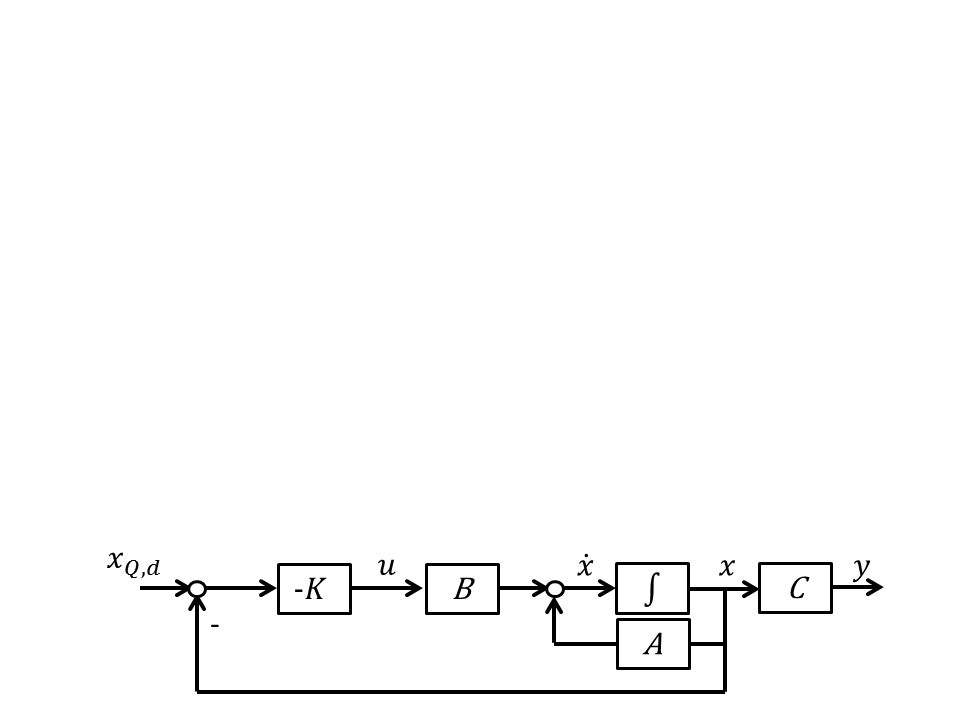
\includegraphics[trim={2cm 0 2cm 14cm},clip,width=.65\textwidth]{./StyleStuff/lqr.png}}
	\caption{LQR control design\label{fig:set.lqr}}
\end{figure}

\a{lqr} control is based on a small angle assumption. 
Therefore, following a traditional modeling method, the rotation matrix is represented with a local coordinate system, 
%Therefore, a traditional modeling method may represent the rotation matrix with a local coordinate system, 
for example with an Euler Angle parameterization. 
The implemented \a{lqr} design is shown in Figure \ref{fig:set.lqr}.\\
A continuous time linearized model of the system used in this controller is represented in the following form 
\begin{align}\label{eq:ss}
\mathbf{\dot{x} }&=A\mathbf{x}+Bu\\
y&=C\mathbf{x}+Du
\end{align}
where $ \mathbf{x} $ is the state vector and $ u $ is the input vector, defined as follows
\begin{equation}\label{eq:state}
\begin{aligned}
%	\textbf{x}&=\begin{bmatrix}
%		\textbf{q}\\
%		\mathbf{\dot{q}}
%	\end{bmatrix}\\
%	\mathbf{q}&=\begin{bmatrix}
%		x&y&z&\phi&\theta&\psi&\phi_L&\theta_L
%	\end{bmatrix}^T\\
%	\mathbf{\dot{q}}&=\begin{bmatrix}
%		\dot{x}&\dot{y}&\dot{z}&\dot{\phi}&\dot{\theta}&\dot{\psi}&\dot{\phi}_L&\dot{\theta}_L
%	\end{bmatrix}^T\\
\mathbf{x}&=\begin{bmatrix}
x&y&z&\phi&\theta&\psi&\phi_L&\theta_L&\dot{x}&\dot{y}&\dot{z}&\dot{\phi}&\dot{\theta}&\dot{\psi}&\dot{\phi}_L&\dot{\theta}_L
\end{bmatrix}^T\\
u&=\begin{bmatrix}
f&M_\phi&M_\theta&M_\psi
\end{bmatrix}^T
\end{aligned}
\end{equation}

Using \texttt{Matlab} command \texttt{lqr(A,B,Q,R)}, an optimal gain matrix $ K $ is calculated, such that the state-feedback law $ u=-K(\mathbf{x-x_{ref}}) $ \cite{Reyes-Valeria2013} minimizes the quadratic cost function. Where the cost function is defined as 
\begin{equation}\label{key}
J(u)=\int_{0}^{\infty}(\mathbf{x}^TQ\mathbf{x}+u^TRu)dt
\end{equation}
%where $ Q $ and $ R $ denote weight matrices that penalize the states and inputs in the cost function. 
The weight matrices $ Q $ and $ R $ define the effects of the states and inputs in the cost function, and the gain matrix $K $ can be calculated. 
The derivation of the state space matrices $ A, B, C, D $, the weight matrices $ Q,R $ and the calculated gain matrix $ K $ can be found in Section \ref{app:lqr}. 

\newpage
\section{Results}\label{sec:exp.results}
In this section the results of the experiments are discussed, for each case separately. 
%Figures \ref{fig:set.caseAres}, \ref{fig:set.caseBres} and \ref{fig:set.caseCres} show 
The load tracking performance for the nonlinear geometric controller is discussed by analyzing the desired and actual load trajectories,   
%The desired load trajectories $ x_{L,d} $ and actual load trajectories $ x_L $ are shown, 
together with the corresponding load position and velocity errors.\\
%$ e_x $ and velocity error $ e_v $.\\ 
The configuration errors $ \Psi_R, \Psi_q $ and the corresponding tracking errors of the \a{qr} attitude $ e_R, e_\Omega $, load attitude $ e_q, e_{\dot{q}} $ are presented.
The error dynamics are analyzed through the error functions, as described in Chapter \ref{ch:control}. 
The stability of the closed-loop system is investigated by observing whether 
%the controller is able 
the zero equilibrium of the closed loop tracking error $(e_x,e_v,e_q,e_{\dot{q}},e_R,e_\Omega)=(0,0,0,0,0,0) $ is exponentially stable.
%, which indicates that the controller is capable of 
%to bring the system to a stationary final state.
%If the required initial conditions are satisfied
%Figures \ref{fig:set.caseAres2}, \ref{fig:set.caseBres2} and \ref{fig:set.caseCres2} show 
\\%, which can be analyzed to check the system's stability.\\
Finally, the load position tracking results of the nonlinear geometric controller and a \a{lqr} controller are compared.
%Figures \ref{fig:set.caseAres3}, \ref{fig:set.caseBres3} and \ref{fig:set.caseCres3} show the differences in controller performance.
%
%
%***************************************\\
%Bart: Suggestie: Misschien een section analysis zou kunnen hepen.. Daarin kun je ook vermelden dat je de percentage error bekijkt etc. 
%Ik lees in deze alinea bijv. dat de NGC en LQR worden vergeleken: op dit punt denk ik dan, ja maar wat wa t wordt er dan precies vergeleken en wordt dat genoemd in de voorgaande sections. Een analysis section zou dat dan kunnen beschrijven.\\
%Nam: Daar had ik Section \ref{sec:exp.proc} voor in gedachte. Eerste alinea aangepast. Voldoende?
%
%***************************************\\

\subsection*{Case A}
In this case, the desired trajectory was shaped like a smooth step-like function to investigate the response of the system to a sudden input.
The desired and actual load position, velocity and acceleration are shown in Figure \ref{fig:AxL} and \ref{fig:AdxL}. 
\begin{figure}[h!]
	\centering
	\makebox[.49\textwidth][c]{\subfloat[][]{\includegraphics[width=.49\textwidth]{\dir{LPOSQRL-xL\caseA}}\label{fig:AxL}}}	
	\makebox[.49\textwidth][c]{\subfloat[][]{\includegraphics[width=.49\textwidth]{\dir{LPOSQRL-dxLd-ddxLd\caseA}}\label{fig:AdxL}}}
	%	\makebox[.49\textwidth][c]{\subfloat[][]{\includegraphics[width=.49\textwidth]{\dir{LPOSQRL-exL\caseA}}\label{fig:AexL}}}
	\caption{Load Position Tracking \a{ngc} Case A \label{}}
\end{figure}

%\begin{figure}[h!]
%	\centering
%	\makebox[.49\textwidth][c]{{\includegraphics[width=.49\textwidth]{\dir{LPOSQRL-dxLd-ddxLd\caseA}}\label{fig:AdxL}}}	
%	\caption{Load Velocity and Acceleration Case A\label{fig:}}
%\end{figure}
Since this function is different from a normal step function, it might be less meaningful to say something about the rise time. 
Normally one checks the time it takes to reach $ 90\% $ of the step height. 
In this case, the step is a smooth function, meaning that the system is not forced to the step height instantly, but in a smooth manner. 
%\begin{figure}[b]
%	\centering
%	\makebox[.49\textwidth][c]{{\includegraphics[width=.49\textwidth]{\dir{LPOSQRL-exL\caseA}}\label{fig:AexL}}}
%	\caption{Load Position Tracking \a{ngc} Case A \label{}}
%\end{figure}
However, it can be seen in Figure \ref{fig:AexLdlqr} that the required time such that $ 90 \% $ of the desired value is reached for the first time is $ 0.61 s $.
It can be observed that the system responds with approximately $ 15 \% $ overshoot in the y-direction, and loses height during this maneuver.
This was to be expected due to large \a{qr} rotations. The error remains within a $ 5 \% $ error bound after $ 1.26 s $, 
to eventually reach a steady-state at the step size of $ 0.25 m $. 
%\clearpage
The load position and velocity error are shown in Figure \ref{fig:AexL}, where Figure \ref{fig:AeR} and \ref{fig:Aeq} show the tracking errors of the \a{qr} attitude and load attitude, respectively. 
The error in \a{qr} attitude and angular velocity are large at the moments the slope starts and ends, indicating the required sudden \a{qr} rotation and high angular velocity are larger than the system can manage.
%to respond to the sudden input. 
Nevertheless, the figures indicate that the errors in both \a{qr} and load attitude are driven to zero relatively fast.

%The figures show that $ (e_x,e_v)=(0,0) $ is exponentially attractive. 
% \\
%From this can be observed that there exist constants $ \alpha,\beta>0 $ for both $ \Psi_R $ and $ \Psi_q $, such it holds that $ \leq min\left\lbrace 2,\alpha e^{-\beta t}\right\rbrace $
%Observations: there exist constants $ \alpha_q,\beta_q>0 $ such that
%\begin{equation}\label{key}
%\Psi_q(q(t),q_d(t)) \leq min\left\lbrace 2,\alpha e^{-\beta t}\right\rbrace 
%\end{equation}
\begin{figure}[h!]
	\centering
	\makebox[.49\textwidth][c]{\subfloat[][]{\includegraphics[width=.49\textwidth]{\dir{LPOSQRL-eR\caseA}}\label{fig:AeR}}}	
	\makebox[.49\textwidth][c]{\subfloat[][]{\includegraphics[width=.49\textwidth]{\dir{LPOSQRL-eq\caseA}}\label{fig:Aeq}}}	
	\makebox[.49\textwidth][c]{\subfloat[][]{\includegraphics[width=.49\textwidth]{\dir{LPOSQRL-exL\caseA}}\label{fig:AexL}}}	
	\caption{Error functions \a{ngc} Case A \label{}}
\end{figure}	

Furthermore, Figure \ref{fig:APsiR} and \ref{fig:APsiq} show that the tracking error functions of the \a{qr} and load, respectively, are also driven to zero.
From this can be concluded that $(e_x,e_v,e_q,e_{\dot{q}},e_R,e_\Omega)=(0,0,0,0,0,0) $ is exponentially stable. 
\begin{figure}[h]
	\centering
	\makebox[.49\textwidth][c]{\subfloat[][]{\includegraphics[width=.49\textwidth]{\dir{LPOSQRL-PsiR\caseA}}\label{fig:APsiR}}}
	\makebox[.49\textwidth][c]{\subfloat[][]{\includegraphics[width=.49\textwidth]{\dir{LPOSQRL-Psiq\caseA}}\label{fig:APsiq}}}
	\caption{Tracking Error functions \a{ngc} Case A \label{}}
\end{figure}	

%***************************************\\
%Bart: Srry dat ik hem even kwijt ben (t is al laat :p), maar je wil toch QR load position tracken. Wat is hier dan de error in QR attitude en load attitude? Deze willen we toh niet tracken?\\
%Nam: Klopt, deels. Maar om het geheel stabiel te houden moeten deze waardes wel naar nul gebracht worden. Dus, dit concludeert dat het systeem closed-loop stabiel is. Onderbelicht of nu wel duidelijk?
%
%Bart: Nu je dit zegt is het wuidelijk, maar het platje is niet betrokken bij je stability check, vandaar een beeetje verwarrend\\
%Nam: Meer toegelicht in procedure. Voldoende?
%
%***************************************\\
For both control approaches, Figure \ref{fig:AxLlqr} shows the load position and Figure \ref{fig:AexLlqr} shows the corresponding load position error. 
Figure \ref{fig:AexLdlqr} shows the absolute position error over the desired load position in percentages. 
From this can be observed that for the \a{lqr} controller the required time to reach $ 90\% $ of the desired value for the first time is $ 1.36 s $. The system responds with approximately $ 23\% $ overshoot and the error remains within a $ 5\% $ error bound after $ 4.75 s $.
Compare to the results of the \a{ngc}, the response is slower, the overshoot is much larger and the settling time is higher.
\newpage
Due to the aggressive maneuver by the \a{ngc} control, the system has a steady-state offset in height. It was found that this can be resolved by tuning the controller with smaller gains or decreasing the cut-off frequency of the low pass filters, which both result in smoother, but slower responses.
\newpage

\begin{figure}[h!]
	\centering
	\makebox[.49\textwidth][c]{\subfloat[][ \label{fig:AxLlqr}]{\includegraphics[width=.49\textwidth]{\dir{LQR-xL\caseA}}}}
	\makebox[.49\textwidth][c]{\subfloat[][\label{fig:AexLlqr}]{\includegraphics[width=.49\textwidth]{\dir{LQR-exL\caseA}}}}	
%	\makebox[.49\textwidth][c]{\subfloat[][Load Position Error Percentage\label{fig:AexLdlqr}]{\includegraphics[width=.49\textwidth]{\dir{LQR-exL_xLd\caseA}}}}		
	\caption{Controller Comparison Case A. Solid: \a{ngc}, Dash-dot: \a{lqr}\label{fig:set.caseAres3}}	
\end{figure}

\begin{figure}[h!]
	\centering
%	\makebox[.49\textwidth][c]{\subfloat[][ \label{fig:AxLlqr}]{\includegraphics[width=.49\textwidth]{\dir{LQR-xL\caseA}}}}
%	\makebox[.49\textwidth][c]{\subfloat[][\label{fig:AexLlqr}]{\includegraphics[width=.49\textwidth]{\dir{LQR-exL\caseA}}}}	
	\makebox[.49\textwidth][c]{{\includegraphics[width=.49\textwidth]{\dir{LQR-exL_xLd\caseA}}}}		
	\caption{Load Position Error Percentage Case A. Solid: \a{ngc}, Dash-dot: \a{lqr}\label{fig:AexLdlqr}}	
\end{figure}
\newpage
Figure \ref{fig:AQRang} shows the \a{qr} attitude with respect to \IF, and a huge difference in the \a{qr} rotations during the maneuver can be observed, note the difference in scale. It is obvious that the \a{ngc} controller is capable of handling more aggressive maneuvers. Figure \ref{fig:ALang} shows the load angle with respect to \IF. The \a{ngc} controller allows larger angles of the load attitude, while stabilization is reached relatively fast. The \a{lqr} controller tries to minimize the swing along the entire trajectory, not allowing large angles of the load attitude. It can be observed that the \a{lqr} controller requires more time to stabilize the load angle, whereas the \a{ngc} controller is capable of damping the oscillation in a smooth manner.
\begin{figure}[h!]
	\centering
	\makebox[.49\textwidth][c]{\subfloat[][\label{fig:AQRang}]{\includegraphics[width=.49\textwidth]{\dir{LQR-QRang\caseA}}}}
	\makebox[.49\textwidth][c]{\subfloat[][\label{fig:ALang}]{\includegraphics[width=.49\textwidth]{\dir{LQR-Lang\caseA}}}}	
	\caption{Controller Comparison Case A. Solid: \a{ngc}, Dash-dot: \a{lqr}\label{fig:set.caseAres4}}	
\end{figure}

\clearpage
%***************************************\\
%%CHECK
%Bart: Is er niet net als bij simpel PID een integrator die de ss fout eruit kan halen zonder je response verder te verslechteren?\\
%Nam: Heb ik wel ergens over gelezen, maar dat vereist een heel andere controller erbij. Om de een of andere reden heb ik er alleen bij de step response last van. Bovendien is het maar 1.5 mm steady state error. Is dat uberhaupt significant?
%
%***************************************\\
%
%
%***************************************\\
%Bart: Waarom ziet jouw controller niet die kleine error en lost hij die uiteindelijk op? hij wil de position error toch naar nul hebben. Dus je hebt een kleine error -> je control output is iets verhoogt -> je actuators zijn ietsje actief -> dus langzaam verwdwijnt de error. Er is toch geen stick slip aar jouw systeem op hangt als bij een pid zonder I?\\
%Nam: Er is zeker geen stick slip in mijn model. Dan zou ik de rotor dynamics ook nog eens moeten modeleren. Ik heb geprobeerd de gain te verhogen op de positie controller, maar het systeem reageert dan heel heftig op voorgaande error, maar niet significant meer op de steady state error. Ik heb echt geen flauw benul hoe het kan.
%
%***************************************\\
\newpage
\subsection*{Case B}
In this case, the desired trajectory was designed to investigate the response of the system to increasing distance and velocities between the ends of a swinging motion.
The desired and actual load position, velocity and acceleration are shown in Figure \ref{fig:BxL} and \ref{fig:BdxL}. 
The corresponding load position and velocity error are shown in Figure \ref{fig:BexL}.
Despite the fact that case B requires higher velocities than in case A, the distance of the load position gradually increases, which requires less sudden aggressive commanded rotations. It can be seen that acceleration in case B is a lot smoother than in case A, which explains why also both the velocity and position are smooth enough for the system to track.
\begin{figure}[h!]
	\centering
	\makebox[.49\textwidth][c]{\subfloat[][]{\includegraphics[width=.49\textwidth]{\dir{LPOSQRL-xL\caseB}}\label{fig:BxL}}}	
	\makebox[.49\textwidth][c]{\subfloat[][]{\includegraphics[width=.49\textwidth]{\dir{LPOSQRL-dxLd-ddxLd\caseB}}\label{fig:BdxL}}}		
	\makebox[.49\textwidth][c]{\subfloat[][]{\includegraphics[width=.49\textwidth]{\dir{LPOSQRL-exL\caseB}}\label{fig:BexL}}}	
	\caption{Load Position Tracking nonlinear geometric control Case B \label{fig:set.caseBres}}
\end{figure}	
%\begin{figure}[h!]
%	\centering
%	\makebox[.49\textwidth][c]{{\includegraphics[width=.49\textwidth]{\dir{LPOSQRL-dxLd-ddxLd\caseB}}\label{fig:BdxL}}}	
%	\caption{Load Velocity and Acceleration Case B\label{fig:}}
%\end{figure}

Figure \ref{fig:BeR} and \ref{fig:Beq} show the tracking errors of the \a{qr} attitude and load attitude, respectively. The error in \a{qr} attitude and angular velocity is much smaller compared to the results in case A, which indicates that the system is fast enough to respond to the required \a{qr} rotations and velocities.
\newpage
\begin{figure}[h!]
	\centering
	\makebox[.49\textwidth][c]{\subfloat[][]{\includegraphics[width=.49\textwidth]{\dir{LPOSQRL-eR\caseB}}\label{fig:BeR}}}	
	\makebox[.49\textwidth][c]{\subfloat[][]{\includegraphics[width=.49\textwidth]{\dir{LPOSQRL-eq\caseB}}\label{fig:Beq}}}	
	\caption{Error functions \a{ngc} Case B \label{}}
\end{figure}	

Both \a{qr} and load attitude errors stay bounded during the trajectory and are driven to zero. 
Furthermore, Figure \ref{fig:BPsiR} and \ref{fig:BPsiq} show a gradual increase and decrease in error, similar to the profile of the desired velocity. 
All error functions are driven to zero, and it can also be concluded for this case that $(e_x,e_v,e_q,e_{\dot{q}},e_R,e_\Omega)=(0,0,0,0,0,0) $ is exponentially stable. 
\begin{figure}[h!]
	\centering
	\makebox[.49\textwidth][c]{\subfloat[][]{\includegraphics[width=.49\textwidth]{\dir{LPOSQRL-PsiR\caseB}}\label{fig:BPsiR}}}
	\makebox[.49\textwidth][c]{\subfloat[][]{\includegraphics[width=.49\textwidth]{\dir{LPOSQRL-Psiq\caseB}}\label{fig:BPsiq}}}
	\caption{Tracking Error functions \a{ngc} Case B \label{}}
\end{figure}	

Figure \ref{fig:BxLlqr} shows the load position for both control approaches. The shape of the actual load position appears to be quite similar. However, taking a look at Figure \ref{fig:BexLlqr} shows the load position error for both control approaches. It is clear that the \a{lqr} controller fails to track the load position, since errors can be seen to reach values up to $ 1.1 m $. 

%***************************************\\
%%CHECK
%Bart: waarom is lijken ze zo op elkaar. De LQR zou de QR angle toch niet naar grote hoeken sturen? Dat is meer een dicussiepunt\\
%Nam:Onderstaand toegevoegd
%
%***************************************\\
The profiles of the \a{qr} rotation angles look notably alike, as can be seen in Figure \ref{fig:BQRang}. 
It shows that the \a{lqr} controller is certainly capable of controlling the \a{qr} to large rotations. 
The gradually increasing velocity allows the \a{lqr} controller to reach larger angles.
However, it can be seen in Figure \ref{fig:BLang} that the load swings significantly more when controlled by the \a{lqr}. 
The load continues its natural swing, which increases the error even more.  
This shows that the \a{lqr} controller struggles with both keeping up with the position and minimizing the load swing.
%The controller is too slow to correct for the \a{qr} position and not capable of correcting the load position error.\\ 
\begin{figure}[h!]
	\centering
	\makebox[.49\textwidth][c]{\subfloat[][\label{fig:BxLlqr}]{\includegraphics[width=.49\textwidth]{\dir{LQR-xL\caseB}}}}
	\makebox[.49\textwidth][c]{\subfloat[][\label{fig:BexLlqr}]{\includegraphics[width=.49\textwidth]{\dir{LQR-exL\caseB}}}}	
%		\makebox[.49\textwidth][c]{\subfloat[][load Position Error Percentage\label{fig:BexLdlqr}]{\includegraphics[width=.49\textwidth]{\dir{LQR-exL_xLd\caseB}}}}	
	\caption{Controller Comparison Case B. Solid: \a{ngc}, Dash-dot: \a{lqr}\label{fig:}}
\end{figure}	
\begin{figure}[h!]
	\centering
	\makebox[.49\textwidth][c]{\subfloat[][\label{fig:BQRang}]{\includegraphics[width=.49\textwidth]{\dir{LQR-QRang\caseB}}}}
	\makebox[.49\textwidth][c]{\subfloat[][\label{fig:BLang}]{\includegraphics[width=.49\textwidth]{\dir{LQR-Lang\caseB}}}}
	%	\makebox[.49\textwidth][c]{\subfloat[][load Position Error Percentage\label{fig:BexLdlqr}]{\includegraphics[width=.49\textwidth]{\dir{LQR-exL_xLd\caseB}}}}	
	\caption{Controller Comparison Case B. Solid: \a{ngc}, Dash-dot: \a{lqr}\label{fig:}}
\end{figure}	

It is also notable that the shape of the load trajectory is nearly correct, this can be explained due to the regular shape of the trajectory and the natural swing of the load. 
It is easily illustrated that the controller has large load position errors due to the swing of the load, when the desired load trajectory becomes more complex.
\newpage
An irregular shape for the desired load trajectory can be created by multiplying the desired load position from this case with a sine wave of an other frequency. 
The signal C in Figure \ref{fig:set.sinecaseB} gets multiplied with signal D to obtain signal E, see Figure \ref{fig:set.sinecaseBB}. The corresponding desired position, velocity and acceleration is shown in Figure \ref{fig:set.xLdcaseBB}.
\begin{figure}[h!]
	\centering
	\makebox[.49\textwidth][c]{\subfloat[][Trajectory generation\label{fig:set.sinecaseBB}]{\includegraphics[width=.45\textwidth]{\dir{LPOSQRL-sineCaseBB\caseBB}}}}	\makebox[.49\textwidth][c]{\subfloat[][Desired trajectory \label{fig:set.xLdcaseBB}]{\includegraphics[width=.45\textwidth]{\dir{LPOSQRL-allxLd\caseBB}}}}
	%	\makebox[.49\textwidth][c]{\subfloat[][ \label{fig:}]{\includegraphics[width=.45\textwidth]{\dir{LPOSQRL-xLdesplot\caseB}}}}
	\caption{Desired load trajectory case B extended, y-direction\label{fig:}}
\end{figure}		

Figure \ref{fig:BBxLlqr} shows the load position and it can be seen that the swinging motion of the actual trajectory is no longer similar to the desired trajectory. 
Figure \ref{fig:BBexLlqr} shows the corresponding load position error.
In Figure \ref{fig:BBQRang} can be seen that the \a{lqr} controller does not react to the large load angles, seen in Figure \ref{fig:BBLang}. The \a{ngc} shows fast changes in the \a{qr} angles to correct for the load position errors.
\begin{figure}[h!]
	\centering
	\makebox[.49\textwidth][c]{\subfloat[][\label{fig:BBxLlqr}]{\includegraphics[width=.49\textwidth]{\dir{LQR-xL\caseBB}}}}
	\makebox[.49\textwidth][c]{\subfloat[][\label{fig:BBexLlqr}]{\includegraphics[width=.49\textwidth]{\dir{LQR-exL\caseBB}}}}	
%	\makebox[.49\textwidth][c]{\subfloat[][\label{fig:BBQRang}]{\includegraphics[width=.49\textwidth]{\dir{LQR-QRang\caseBB}}}}
%\makebox[.49\textwidth][c]{\subfloat[][\label{fig:BBLang}]{\includegraphics[width=.49\textwidth]{\dir{LQR-Lang\caseBB}}}}
	\caption{Controller Comparison Case B extended. Solid: \a{ngc}, Dash-dot: \a{lqr}\label{fig:}}
\end{figure}	
\begin{figure}[t]
	\centering
%	\makebox[.49\textwidth][c]{\subfloat[][\label{fig:BBxLlqr}]{\includegraphics[width=.49\textwidth]{\dir{LQR-xL\caseBB}}}}
%	\makebox[.49\textwidth][c]{\subfloat[][\label{fig:BBexLlqr}]{\includegraphics[width=.49\textwidth]{\dir{LQR-exL\caseBB}}}}	
	\makebox[.49\textwidth][c]{\subfloat[][\label{fig:BBQRang}]{\includegraphics[width=.49\textwidth]{\dir{LQR-QRang\caseBB}}}}
	\makebox[.49\textwidth][c]{\subfloat[][\label{fig:BBLang}]{\includegraphics[width=.49\textwidth]{\dir{LQR-Lang\caseBB}}}}
	\caption{Controller Comparison Case B extended. Solid: \a{ngc}, Dash-dot: \a{lqr}\label{fig:}}
\end{figure}	

\clearpage

\newpage
\subsection*{Case C}
The last case is designed to investigate the response to a more complex desired load trajectory in three directions, each direction with a different shape. 
The desired and actual load position, velocity and acceleration are shown in Figure \ref{fig:CxL} and \ref{fig:CdxL}. 
%The corresponding load position and velocity error are shown in Figure \ref{fig:CexL}. 
\begin{figure}[h!]
	\centering
	\makebox[.495\textwidth][c]{\subfloat[][]{\includegraphics[width=.49\textwidth]{\dir{LPOSQRL-xL\caseC}}\label{fig:CxL}}}	
	\makebox[.495\textwidth][c]{\subfloat[][]{\includegraphics[width=.49\textwidth]{\dir{LPOSQRL-dxL\caseC}}\label{fig:CdxL}}}	
		\makebox[.49\textwidth][c]{\subfloat[][]{\includegraphics[width=.49\textwidth]{\dir{LPOSQRL-exL\caseC}}\label{fig:CexL}}}	
	
	\caption{Load Position Tracking nonlinear geometric control Case C \label{fig:set.caseCres}}
\end{figure}	

As can be seen in Figure \ref{fig:CexL}, the error in height is quite large. 
This can be explained by the combination of height loss due to rotation and the changing desired height trajectory. 
At some point in time the load is required to fly a distance of $ 2 m $ from side to side in the y-direction with approximately $ 2 m/s $. 
At the same time when the \a{qr} is inclined, the trajectory in the z-direction requires the load to go up and down. 

%The control gains that were used in Case B, resulted in large errors in this case, see \ref{tab:set.gains}.
%It could be seen that the system reacted to aggressively by calculating huge commanded signals. 
%For that reason the controller gains were lowered to prove the concept of the geometric controller, resulting in slower, but smoother responses. 

As expected, the \a{qr} loses height due to a decreasing total upward force whenever the \a{qr} is inclined.
The error in the y-direction is most likely the result of the increasing required speed in both the x- and y-direction.
The \a{qr} is capable of creating a moment around a body axis. 
However, when the \a{qr} is rotated around one body axis, a rotation around the other body axis will not result in a straight translation.
This makes it challenging to move fast in one direction while swinging perpendicular to that direction.
%Furthermore it must be mentioned that the control gains used for Case B, would result

%
%Figure \ref{fig:CeR} and \ref{fig:Ceq} show the tracking errors of the \a{qr} attitude and load attitude, respectively. \\
%Observations: $(e_x,e_v,e_q,e_{\dot{q}},e_R,e_\Omega)=(0,0,0,0,0,0) $ is exponentially stable.

Despite the errors, the \a{qr} is able to stabilize the system to an equilibrium, this can be seen in Figures \ref{fig:CexL}, \ref{fig:CeR}, \ref{fig:Ceq}, \ref{fig:CPsiR} and \ref{fig:CPsiq}. It can be observed that $(e_x,e_v,e_q,e_{\dot{q}},e_R,e_\Omega)=(0,0,0,0,0,0) $ is exponentially stable.

\begin{figure}[h!]
	\centering
	\makebox[.49\textwidth][c]{\subfloat[][]{\includegraphics[width=.49\textwidth]{\dir{LPOSQRL-eR\caseC}}\label{fig:CeR}}}	
	\makebox[.49\textwidth][c]{\subfloat[][]{\includegraphics[width=.49\textwidth]{\dir{LPOSQRL-eq\caseC}}\label{fig:Ceq}}}	
		\caption{Error functions \a{ngc} Case C \label{}}
\end{figure}	
\begin{figure}[h!]
	\centering
	\makebox[.49\textwidth][c]{\subfloat[][]{\includegraphics[width=.49\textwidth]{\dir{LPOSQRL-PsiR\caseC}}\label{fig:CPsiR}}}
	\makebox[.49\textwidth][c]{\subfloat[][]{\includegraphics[width=.49\textwidth]{\dir{LPOSQRL-Psiq\caseC}}\label{fig:CPsiq}}}
	\caption{Tracking Error functions \a{ngc} Case C \label{}}
\end{figure}	

Figure \ref{fig:CxLlqr} shows the load position and Figure \ref{fig:CexLlqr} shows the load position error for both control approaches. 
It is evident that the \a{lqr} controller is not suitable for load position tracking of such complex trajectories. 
%
%Comparable to case B, the shape of the actual load position is quite similar. However,  for both control approaches.
%It is not surprising that the \a{lqr} controller fails again to track the load position, for the trajectory is more complex than the other cases. 
\begin{figure}[h!]
	\centering
	\makebox[.49\textwidth][c]{\subfloat[][  \label{fig:CxLlqr}]{\includegraphics[width=.49\textwidth]{\dir{LQR-xL\caseC}}}}
	\makebox[.49\textwidth][c]{\subfloat[][  \label{fig:CexLlqr}]{\includegraphics[width=.49\textwidth]{\dir{LQR-exL\caseC}}}}
	\caption{Controller Comparison Case C. Solid: \a{ngc}, Dash-dot: \a{lqr}\label{fig:set.}}
\end{figure}	

Figure \ref{fig:CQRang} and \ref{fig:CLang} show the \a{qr} and load angle w.r.t. \IF. The main difference that can be observed are the spikes in the \a{ngc} approach. The \a{ngc} \a{qr} attitude controller is able to calculate the required rotation along the trajectory, based on the error information. 
This indicates fast maneuvering, something what the \a{lqr} controller is not capable of. 
\newpage
% 
%The commands that are sent by the \a{lqr} results in a smooth response, but
%sends smooth commands to the system, resulting in a 
% in a smooth
%In Figure  the load angle with respect to \BF is shown. 
The load angle by \a{ngc} has a peculiar shape, for it is not a smooth sine-wave like shape. The pointy almost triangular shapes indicate that load angle is controlled actively, rather than letting it swing freely. This can be related to the peaks in the \a{qr} angle, see Figure \ref{fig:CQRang}. 
\begin{figure}[h!]
	\centering
	\makebox[.49\textwidth][c]{\subfloat[][\label{fig:CQRang}]{\includegraphics[width=.49\textwidth]{\dir{LQR-QRang\caseC}}}}
	\makebox[.49\textwidth][c]{\subfloat[][\label{fig:CLang}]{\includegraphics[width=.49\textwidth]{\dir{LQR-Lang\caseC}}}}
	\caption{Controller Comparison Case C. Solid: \a{ngc}, Dash-dot: \a{lqr}\label{fig:set.}}
\end{figure}	
\clearpage

\newpage
\section{Summary}\label{set:exp.con}
This chapter describes the experiments to test the nonlinear geometric controller on its ability to track load trajectories. 
It is explained how the stability of the system and the load position tracking performance can be analyzed. 

The first trajectory is a smooth step-like function, which allows properties similar in the analysis of a step response to be observed.
Next, the second trajectory describes an increasing load position trajectory to investigate the systems response on tracking a load trajectory with increasing velocities.
Finally, the last trajectory describes a three-dimensional load position tracking task, by generating a complex trajectories to test the response to limitations of the system. 

Matlab and Simulink were used to create simulations of the experiments, and data was generated to analyze the responses of the system. 
Along with the chosen parameters, the results of the experiments are presented.
The experiments were done with both the nonlinear geometric controller and an \a{lqr} controller.
Differences in the control performances were discussed and the concept of the nonlinear geometric controller is proven.




